\documentclass{article}[12 pt]
\usepackage{customDecorator}
\usepackage{amsmath}
\usepackage{amssymb}
\usepackage{float}
\usepackage{subcaption}

\usepackage{tikz}
\usetikzlibrary{arrows,datavisualization.formats.functions,external}
\tikzexternalize[prefix=figures/]

\tikzset{
hollow node/.style={draw, circle,fill=white, minimum width=5pt, inner sep=0pt},
    black node/.style={draw, circle, fill=black, inner sep=0pt,
    minimum width=5pt}
}

\newcommand{\grapha}[3]{
\begin{tikzpicture}[scale=2]
  \datavisualization [school book axes,
    visualize as smooth line/.list={one},
    y axis={label={#3}},
    x axis={label={$t$}},
    one={style={black}},  
  ]

    data [set=one,format=function] {
        var x : interval [-#1:3];
        func y = exp(-2* (\value x+#1));
    };
    info{
    \node at (-#1+.4,0.4) [anchor=south west] {#2};
    };
    \draw [] (-#1,0) -- (-#1,1);
    
\end{tikzpicture}
}

\newcommand{\graphb}[6]{
\begin{tikzpicture}
    \datavisualization [school book axes,
    visualize as smooth line/.list={one,two},
    y axis={label={#6}, ticks={major={at={0}}}},
    x axis={label={$t$}, ticks={major={at={}}}},
    one={style={black}},
    two={style={black}}    
  ]

    data [set=one,format=function] {
        var x : interval [0:#1*3];
        func y = 2*exp(#4* \value x);
    }

    data [set=two,format=function] {
        var x : interval [-1.5*#1:0];
        func y = 2;
    };
    info{
    \node at (#1*1.5,1) [anchor=south west] {#5};
   \node at (0,2) [anchor=south east] {\small{$2$}};
   \node at (#2,0) [anchor=north] {\small{#2}};
   \node at (#3,0) [anchor=north east] {\small{#3}};
    };
    \draw [] (-1.5*#1,0) -- (-1.5*#1,2);
    \draw [] (3*#1,0) -- (3*#1,0.4462603203);
\end{tikzpicture}
}


\newcommand{\graphc}[5]{
\begin{tikzpicture}[scale=1.5]
    \datavisualization [school book axes,
    visualize as smooth line/.list={one,two},
    y axis={label={#4}},
    x axis={label={$t$}},
    one={style={black}}, 
    two={style={black}}, 
  ]

    data [set=one,format=function] {
        var x : interval [#1:#2];
        func y = exp(#3* \value x);
    };
    info{
    \node at (#1+2,0.3) [anchor=south west] {#5};
    };
    \ifnum#1>0
    \draw [] (1,0) -- (1,0.6065306597);
    \else
    \draw [] (-1,0) -- (-1,0.6065306597);
    \fi
\end{tikzpicture}
}


\newcommand{\evenodd}{
\begin{tikzpicture}[scale=2]
\datavisualization [school book axes,
    y axis={label={$x(t)$},ticks={minor={at={0,1,-1,0.5,-0.5}}},max value=1.5, min value=-1.5},
    x axis={label={$t$},ticks={major={at={1,-1}}},max value=1.5, min value=-1.5},
     ]
      info{
  \node at (0,0.5)  [anchor=west]{\small{$0.5$}};
  \node at (0,-0.5)  [anchor=east]{\small{$-0.5$}};
};
   \draw [ultra thick] (-1,0)--(-1,1); 
    \draw [ultra thick] (-1,1)--(0,0.5); 
   \draw [ultra thick] (0,0.5)--(0,-0.5);  
   \draw [ultra thick] (0,-0.5)--(1,0); 
\end{tikzpicture}
}

\newcommand{\evengrapha}{
\begin{tikzpicture}[scale=2]
\datavisualization [school book axes,
    y axis={label={$x(-t)$},ticks={minor={at={0,1,-1,0.5,-0.5}}},max value=1.5, min value=-1.5},
    x axis={label={$t$},ticks={major={at={1,-1}}},max value=1.5, min value=-1.5},
     ]
       info{
  \node at (0,0.5)  [anchor=east]{\small{$0.5$}};
  \node at (0,-0.5)  [anchor=west]{\small{$-0.5$}};
};
   \draw [ultra thick] (-1,0)--(0,-0.5); 
    \draw [ultra thick] (0,-0.5)--(0,0.5); 
   \draw [ultra thick] (0,0.5)--(1,1);  
   \draw [ultra thick] (1,1)--(1,0); 
\end{tikzpicture}
}
\newcommand{\evengraphb}{
\begin{tikzpicture}[scale=2]
\datavisualization [school book axes,
    y axis={label={$x(t)+x(-t)$},ticks={minor={at={0,1,-1,0.5,-0.5}}},max value=1.5, min value=-1.5},
    x axis={label={$t$},ticks={major={at={1,-1}}},max value=1.5, min value=-1.5},
     ];
   \draw [ultra thick] (-1,0)--(-1,1);  
   \draw [ultra thick] (-1,1)--(0,0); 
    \draw [ultra thick] (0,0)--(1,1); 
   \draw [ultra thick] (1,1)--(1,0); 
\end{tikzpicture}
}
\newcommand{\evengraphc}{
\begin{tikzpicture}[scale=2]
\datavisualization [school book axes,
    y axis={label={$x_e=\frac{x(t)+x(-t)}{2}$},ticks={major={at={0,1,-1,0.5,-0.5}}},max value=1.5, min value=-1.5},
    x axis={label={$t$},ticks={major={at={1,-1}}},max value=1.5, min value=-1.5},
     ];
   \draw [ultra thick] (-1,0)--(-1,0.5);  
   \draw [ultra thick] (-1,0.5)--(0,0); 
    \draw [ultra thick] (0,0)--(1,0.5); 
   \draw [ultra thick] (1,0.5)--(1,0); 
\end{tikzpicture}
}
\newcommand{\oddgrapha}{
\begin{tikzpicture}[scale=1.5]
\datavisualization [school book axes,
    y axis={label={$-x(-t)$},ticks={minor={at={0,1,-1,0.5,-0.5}}},max value=1.5, min value=-1.5},
    x axis={label={$t$},ticks={major={at={-1}}},max value=1.5, min value=-1.5},
     ]
       info{
  \node at (0,0.5)  [anchor=west]{\small{$0.5$}};
  \node at (0,-0.5)  [anchor=east]{\small{$-0.5$}};
  \node at (1,0)  [anchor=south]{\small{$1$}};
};
   \draw [ultra thick] (-1,0)--(0,0.5); 
    \draw [ultra thick] (0,0.5)--(0,-0.5); 
   \draw [ultra thick] (0,-0.5)--(1,-1);  
   \draw [ultra thick] (1,-1)--(1,0); 
\end{tikzpicture}
}
\newcommand{\oddgraphb}{
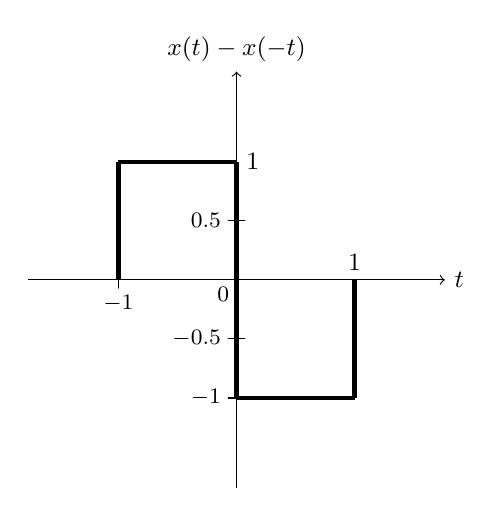
\begin{tikzpicture}[scale=1.5]
\datavisualization [school book axes,
    y axis={label={$x(t)-x(-t)$},ticks={major={at={0,-1,0.5,-0.5}}},max value=1.5, min value=-1.5},
    x axis={label={$t$},ticks={major={at={-1}}},max value=1.5, min value=-1.5},
     ]
       info{
  \node at (0,1)  [anchor=west]{\small{$1$}};
  \node at (1,0)  [anchor=south]{\small{$1$}};
};
   \draw [ultra thick] (-1,0)--(-1,1); 
    \draw [ultra thick] (-1,1)--(0,1); 
   \draw [ultra thick] (0,1)--(0,-1);  
   \draw [ultra thick] (0,-1)--(1,-1); 
   \draw [ultra thick] (1,-1)--(1,0); 
\end{tikzpicture}
}
\newcommand{\oddgraphc}{
\begin{tikzpicture}[scale=1.5]
\datavisualization [school book axes,
    y axis={label={$x_o=\frac{x(t)-x(-t)}{2}$},ticks={minor={at={0,1,-1,0.5,-0.5}}},max value=1.5, min value=-1.5},
    x axis={label={$t$},ticks={major={at={-1}}},max value=1.5, min value=-1.5},
     ]
       info{
  \node at (0,0.5)  [anchor=west]{\small{$0.5$}};
  \node at (0,-0.5)  [anchor=east]{\small{$-0.5$}};
  \node at (1,0)  [anchor=south]{\small{$1$}};
};
   \draw [ultra thick] (-1,0)--(-1,0.5); 
    \draw [ultra thick] (-1,0.5)--(0,0.5); 
   \draw [ultra thick] (0,0.5)--(0,-0.5);  
   \draw [ultra thick] (0,-0.5)--(1,-0.5); 
   \draw [ultra thick] (1,-0.5)--(1,0); 
\end{tikzpicture}
}

\newcommand{\rectContinuous}{
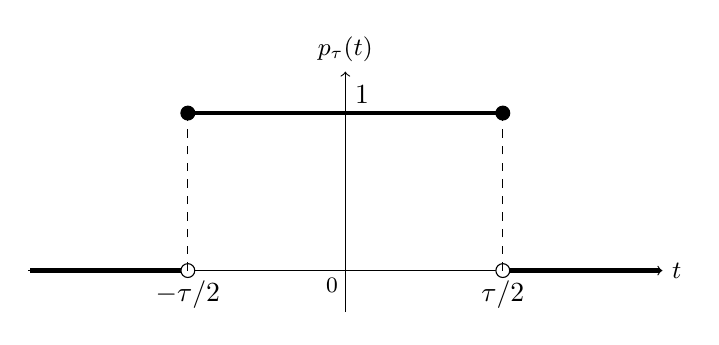
\begin{tikzpicture}[scale=2]
  \datavisualization [school book axes,
    visualize as smooth line/.list={one,two,three},
    y axis={label={$p_\tau(t)$},ticks={major={at={0}}},max value=1, min value=0},
    x axis={label={$t$},ticks={major={at={}}},max value=1.75, min value=-1.75},
    one={style={black, ultra thick}},
    two={style={black, ultra thick}}, 
    three={style={black, ultra thick}}, 
  ]

    data [set=one,format=function] {
        var x : interval [-1:1];
        func y = 1;
    }
    data [set=two,format=function] {
        var x : interval [-2:-1];
        func y = 0;
    }
    data [set=three,format=function] {
        var x : interval [1:2];
        func y = 0;
    };
    info{
  \node at (1,0) [anchor=north] {$\tau/2$};
  \node at (-1,0) [anchor=north] {$-\tau/2$};
  \node at (0,1) [anchor=south west] {$1$};
  \node at (1,0)[hollow node]  {};
  \node at (-1,0)[hollow node]  {};
  \node at (1,1)[black node]  {};
  \node at (-1,1)[black node]  {};
    };
    
    \draw [dashed] (1,0) -- (1,1);
     \draw [dashed] (-1,0) -- (-1,1);
     
\end{tikzpicture}
}

\newcommand{\rectDiscrete}{
\begin{tikzpicture}[scale=2]
  \datavisualization [school book axes,
    y axis={label={$p_\tau[n]$},ticks={major={at={0}}}, max value=1, min value=0},
    x axis={label={$n$},ticks={major={at={}}},max value=2, min value=-2},
  ]

    info{
  \node at (1,0) [anchor=north] {$m/2$};
  \node at (-1,0) [anchor=north] {$-m/2$};
  \node at (0,1) [anchor=south west] {$1$};
  \node at (1,0)[hollow node]  {};
  \node at (-1,0)[hollow node]  {};
\foreach \position in {(-2,0),(-1.5,0),(-1,1),(-0.5,1),(0,1),(0.5,1),(1,1),(1.5,0),(2,0)}
\node at \position [black node]{};
    };
    
    \draw [dashed] (1,0) -- (1,1);
    \draw [dashed] (-1,0) -- (-1,1);
     
\end{tikzpicture}
}

\newcommand{\rampContinuous}{
\begin{tikzpicture}[scale=2]
  \datavisualization [school book axes,
    y axis={label={$r(t)$},ticks={major={at={0}}}, max value=2, min value=0},
    x axis={label={$t$},ticks={major={at={}}},max value=2 , min value=-1.75},
  ];
    
    \draw [ultra thick, ->] (0,0) -- (1.75,1.75);
    \draw [ultra thick] (-2,0) -- (0,0);
     
\end{tikzpicture}
}
\newcommand{\rampDiscrete}{
\begin{tikzpicture}[scale=2]
  \datavisualization [school book axes,
    y axis={label={$r[n]$},ticks={major={at={0}}}, max value=2, min value=0},
    x axis={label={$n$},ticks={major={at={1,2,-1,-2}}},max value=2 , min value=-1.75},
  ];
    info{
\foreach \position in {(-2,0),(-1,0),(0,0),(1,1),(2,2)}
\node at \position [black node]{};
    };
\end{tikzpicture}
}

\newcommand{\signumContinuous}{
\begin{tikzpicture}[scale=2]
  \datavisualization [school book axes,
    y axis={label={$sgn(t)$},ticks={major={at={}}}, max value=1, min value=-1},
    x axis={label={$t$},ticks={major={at={}}},max value=2, min value=-2},
  ]

    info{
  \node at (0,-1)[hollow node]  {};
  \node at (0,1)[hollow node]  {};
  \node at (0,0)[black node]  {};
  \node at (0,1)  [anchor=east]{$1$};
  \node at (0,-1)  [anchor=west]{$-1$};
};
    
    \draw [ultra thick] (0,1) -- (2,1);
    \draw [ultra thick] (0,-1) -- (-2,-1);
     
\end{tikzpicture}
}
\newcommand{\signumDiscrete}{
\begin{tikzpicture}[scale=2]
  \datavisualization [school book axes,
    y axis={label={$sgn[n]$},ticks={major={at={}}}, max value=1, min value=-1},
    x axis={label={$n$},ticks={major={at={}}},max value=2, min value=-2},
  ]
  
    info{
   \node at (0,1)  [anchor=east]{$1$};
   \node at (0,-1)  [anchor=west]{$-1$};
   \foreach \position in {(-2,-1),(-1,-1),(0,0),(1,1),(2,1)}
\node at \position [black node]{};
};
    
    \draw [dashed] (0,1) -- (2,1);
    \draw [dashed] (0,-1) -- (-2,-1);
     
\end{tikzpicture}
}

\newcommand{\ab}[5]{
\begin{equation*}
x\left(#5\right)=\begin{cases}
  2 & #1\leq #2<0\\
  #3 & 0\leq #2<#4\\
  0 & \text{otherwise}
\end{cases}
\end{equation*}
}

\begin{document}
\titlePage{Signal Analysis Assignment \#2}{September 7th, 2020}{Dr. Dibakar Raj Panta}
\begin{problem}{
Find the even and odd components of $x(t)=e^{jt}$.}
\end{problem}
\begin{solution}
{
For any signal $x(t)$ in the continuous time domain, if $x_e(t)$ and $x_o(t)$ represent the even and odd components of that signal, they can be calculated as follows,
\begin{equation*}
\begin{aligned}
x_e(t)&=\frac{1}{2}\left\{x(t)+x(-t)\right\}\\
x_o(t)&=\frac{1}{2}\left\{x(t)-x(-t)\right\}\\
\end{aligned}
\end{equation*} 
The signal we have is, $x(t)=e^{jt}$. So, the time-reversed signal can be written as, $x(-t)=e^{-jt}$.\\
So, from these statements we can figure out the even and odd components of the signal $x(t)$ as,
\begin{equation*}
\begin{aligned}
x_e(t)&=\frac{1}{2}\left\{e^{jt}+e^{-jt}\right\}\\
&=cos(t)\\
x_o(t)&=\frac{1}{2}\left\{e^{jt}-e^{-jt}\right\}\\
&=j\frac{1}{2j}\left\{e^{jt}-e^{-jt}\right\}\\
&=jsin(t)
\end{aligned}
\end{equation*}
Thus, the even and odd components of the signal $x(t)=e^{jt}$ are $cos(t)$ and $jsin(t)$ respectively.
}
\end{solution}
\begin{problem}
{Find the even and odd components of the signal shown in Figure~\ref{fig:evenodd}.\begin{figure}[H]
\centering
\evenodd
\caption{Plot for $x(t)$}
\label{fig:evenodd}
\end{figure}}
\end{problem}
\newpage
\begin{solution}{
For any signal $x(t)$ in the continuous time domain, if $x_e(t)$ and $x_o(t)$ represent the even and odd components of that signal, they can be calculated as follows,
\begin{equation*}
\begin{aligned}
x_e(t)&=\frac{1}{2}\left\{x(t)+x(-t)\right\}\\
x_o(t)&=\frac{1}{2}\left\{x(t)-x(-t)\right\}\\
\end{aligned}
\end{equation*} 
\begin{figure}[H]
\begin{subfigure}{.5\textwidth}
  \centering
  \evengrapha
  \caption{Plot for time-reversed $x(t)$}
  \label{fig:even-first}
\end{subfigure}
\begin{subfigure}{.5\textwidth}
  \centering
  \evengraphb
  \caption{Plot for $x(t)+x(-t)$}
  \label{fig:even-second}
\end{subfigure}
\begin{subfigure}{\textwidth}
  \centering
  \evengraphc
  \caption{Plot for even component of $x(t)$ i.e. $x_e(t)$}
  \label{fig:even-third}
\end{subfigure}
\caption{Plots for determining the even component of $x(t)$}
\label{fig:evengraph}
\end{figure}
\begin{figure}[H]
\begin{subfigure}{.5\textwidth}
  \centering
  \oddgrapha
  \caption{Plot for time-reversed and amplitude-reversed $x(t)$}
  \label{fig:odd-first}
\end{subfigure}
\begin{subfigure}{.5\textwidth}
  \centering
  \oddgraphb
  \caption{Plot for $x(t)-x(-t)$}
  \label{fig:odd-second}
\end{subfigure}
\begin{subfigure}{\textwidth}
  \centering
  \oddgraphc
  \caption{Plot for odd component of $x(t)$ i.e. $x_o(t)$}
  \label{fig:odd-third}
\end{subfigure}
\caption{Plots for determining the odd component of $x(t)$}
\label{fig:oddgraph}
\end{figure}
Figure~\ref{fig:even-third} and Figure~\ref{fig:odd-third} represent the even and odd components of the original signal $x(t)$.
}\end{solution}
\begin{problem}
{An exponential function $x(t)=e^{-2t}$ shown in Figure~\ref{fig:qa} is delayed by 1 second. Sketch and matematically describe the delayed function. Repeat the problem with $x(t)$ advanced by 1 second.
\begin{figure}[H]
\centering
\grapha{0}{$e^{-2t}$}{$x(t)$}
\caption{Plot for $x(t)=e^{-2t}$}
\label{fig:qa}
\end{figure}
}
\end{problem}
\begin{solution}
{
Time-delay and time-advancements are quite necessary transformations of a signal with great significance in communications. Advancing or reflecting a signal is only possible in real-time, whereas for a recorded signal, delay is also possible.\\
A signal $x(t-\tau)$ is said to be delayed in time by a positive value $\tau$ seconds for the original signal $x(t)$. It is to be noted that delaying a signal by $\tau$ seconds means that the original signal has been shifted to the right and the corresponding value of $x(0)$ now exists at $t-\tau=0$ for $x(t-\tau)$. This means the signal $x(t-\tau)$ starts $\tau$ seconds later than $x(t)$ hence beign delayed. Similarly, a signal $x(t+\tau)$ is said to be advanced in time by a positive value $\tau$ seconds for the original signal $x(t)$. The signal is shifted to the left and hence starts before the original signal $x(t)$. The corresponding value of $x(0)$ exists at $t+\tau=0$ for $x(t+\tau)$. This means the signal $x(t+\tau)$ starts $\tau$ seconds earlier than $x(t)$ hence beign advanced.\\\\
It is given that, $x(t)=e^{-2t}$,\\
so for the signal to be time-delayed by 1 second, we have,
\begin{equation*}
x(t-1)=e^{-2(t-1)}
\end{equation*}
This means the signal $x(t)$ is shifted to the right by 1 second. Graphically, this is represented by Figure~\ref{fig:td}.
\begin{figure}[H]
\centering
\grapha{-1}{$e^{-2t+2}$}{$x(t-1)$}
\caption{Plot for $x(t)$ delayed in time by 1 second, i.e. $x(t-1)$ }
\label{fig:td}
\end{figure}
Similarly, for the signal to be time-advanced by 1 second, we have,\begin{equation*}
x(t+1)=e^{-2(t+1)}
\end{equation*}
This means the signal $x(t)$ is shifted to the left by 1 second. Graphically, this is represented by Figure~\ref{fig:ta}.
\begin{figure}[H]
\centering
\grapha{1}{$e^{-2t-2}$}{$x(t+1)$}
\caption{Plot for $x(t)$ advanced in time by 1 second, i.e. $x(t+1)$}
\label{fig:ta}
\end{figure}
}
\end{solution}
\begin{problem}
{Figure~\ref{fig:qb} shows a signal $x(t)$. Sketch and describe mathematically this signal time-compressed by factor 3. Repeat the problem for the same signal time-expanded by factor 2.
\begin{figure}[H]
\centering
\graphb{1}{3}{-1.5}{-0.5}{$2e^{-t/2}$}{$x(t)$}
\caption{Plot for $x(t)$}
\label{fig:qb}
\end{figure}
}
\end{problem}
\begin{solution}{
The signal $x(t)$ can be described as,
\ab{-1.5}{t}{2e^{-t/2}}{3}{t}
The time-compressed result of a signal $x(t)$ by a factor of $k$ is calculated as $x(kt)$. Since the horizontal axis is scaled by a factor of $k$, the resulting signal is time-compressed.\\ Mathematically,
\ab{-1.5}{3t}{2e^{-3t/2}}{3}{3t}
This can be further reduced to get,
\ab{-0.5}{t}{2e^{-1.5t}}{1}{3t}
A plot for the time-compressed signal is shown in Figure \ref{fig:tc}.
\begin{figure}[H]
\centering
\graphb{1/3}{1}{-0.5}{-3/2}{$2e^{-1.5t}$}{$x_c(t)$}
\caption{Plot for $x(t)$ time-compressed by factor 3}
\label{fig:tc}
\end{figure}
Similarly, the time-expanded result of a signal $x(t)$ by a factor of $k$ is calculated as $x(\frac{t}{k})$. Since the horizontal axis is being reduced by a factor of $k$, the resulting signal is time-expanded by the same factor.\\
Mathematically,
\ab{-1.5}{\frac{t}{2}}{2e^{-t/4}}{3}{\frac{t}{2}}
This can be further reduced to get,
\ab{-3}{t}{2e^{-t/4}}{6}{\frac{t}{2}}
A plot for the time-expanded signal is shown in Figure \ref{fig:te}.
\begin{figure}[H]
\centering
\graphb{2}{6}{-3}{-1/4}{$2e^{-t/4}$}{$x_e(t)$}
\caption{Plot for $x(t)$ time-expanded by factor 2}
\label{fig:te}
\end{figure}
}

\end{solution}

\begin{problem}{For the signal $x(t)$, sketch $x(-t)$, which is time-reversed $x(t)$.
\begin{equation*}
x(t)=\begin{cases}
  e^{t/2} & -1\geq t>-5\\
  0 & \text{otherwise}
\end{cases}
\end{equation*}
}\end{problem}
\begin{solution}{A signal $x(-t)$ is said to be time reversed or reflected for the original signal $x(t)$. This is visualized by flipping the sigal $x(t)$ about the origin.\\\\
Mathematically,
\begin{equation*}
\begin{aligned}
x(-t)&=\begin{cases}
  e^{-t/2} & -1\geq -t>-5\\
  0 & \text{otherwise}
\end{cases}\\
x(-t)&=\begin{cases}
  e^{-t/2} & 1\leq t<5\\
  0 & \text{otherwise}
\end{cases}
\end{aligned}
\end{equation*}
This can be simply realized by taking the mirror image of the signal $x(t)$ about the y-axis.
Figure~\ref{fig:tro} represents the original signal $x(t)$ and Figure~\ref{fig:tr} represents the time-reversed signal $x(-t)$ for the given ranges.
\begin{figure}[H]
\centering
\graphc{-5}{-1}{0.5}{$x(t)$}{$e^{t/2}$}
\caption{Plot for $x(t)$}
\label{fig:tro}
\end{figure}
\begin{figure}[H]
\centering
\graphc{1}{5}{-0.5}{$x(-t)$}{$e^{-t/2}$}
\caption{Plot for $x(-t)$}
\label{fig:tr}
\end{figure}
}
\end{solution}
\begin{problem}{Define rectangular pulse, signum function and ramp function both in continuous and discrete time.}\end{problem}
\begin{solution}
{
\textbf{Rectangular Pulse}\\
A rectangular pulse function otherwise known as rectangle function or gate function is simply a function that has an amplitude of A inside a certain internal and 0 otherwise.\\\\
A rectangular pulse in \textbf{continuous time} with a period of $T$ is defined as,
\begin{equation*}
p_\tau(t) \triangleq \begin{cases}
  A & \frac{-LT}{2} \leq t \leq \frac{LT}{2}\\
  0 & \text{otherwise}
\end{cases}
\end{equation*}
Likewise, a unit rectangular pulse with period of $\tau$ centered at (0,0) is defined as,
\begin{equation*}
p_\tau(t) \triangleq \begin{cases}
  1 & \frac{-\tau}{2} \leq t \leq \frac{\tau}{2}\\
  0 & \text{otherwise}
\end{cases}
\end{equation*}
\begin{figure}[H]
\centering
\rectContinuous
\caption{Plot for unit rectangular pulse in continuous time}
\label{fig:rectContinuous}
\end{figure}
Similarly, the discrete version of the rectangular pulse can be obtained by sampling. For $m=2\left(\frac{\tau}{2T}\right)$ where $T$ is the sampling period, a rectangular pulse in \textbf{discrete-time} is defined as,
\begin{equation*}
p_m[n] \triangleq \begin{cases}
  A & \frac{-m}{2} \leq n \leq \frac{m}{2}\\
  0 & \text{otherwise}
\end{cases}
\end{equation*}
A unit rectangular pulse in discrete-time centered at (0,0) is defined as,
\begin{equation*}
p_m[n] \triangleq \begin{cases}
  1 & \frac{-m}{2} \leq n \leq \frac{m}{2}\\
  0 & \text{otherwise}
\end{cases}
\end{equation*}
\begin{figure}[H]
\centering
\rectDiscrete
\caption{Plot for unit rectangular pulse in discrete time}
\label{fig:rectDiscrete}
\end{figure}
\textbf{Signum Function}\\
A signum function is one that has amplitude $+1$ for the positive x-axis, $-1$ for the negative x-axis and $0$ at origin, which is why it is also known as a sign function.\\\\
Mathematically, in \textbf{continuous time domain}, a signum function is defined as,
\begin{equation*}
sgn[t] \triangleq \begin{cases}
  1 & t > 0\\
  0 & t=0\\
  -1 & t<0
\end{cases}
\end{equation*}
\begin{figure}[H]
\centering
\signumContinuous
\caption{Plot for signum function in continuous time}
\label{fig:signumContinuous}
\end{figure}
Similarly, the \textbf{discrete time} version of the signum function is defined as,
\begin{equation*}
sgn[n] \triangleq \begin{cases}
  1 & n > 0\\
  0 & n=0\\
  -1 & n<0
\end{cases}
\end{equation*}
\begin{figure}[H]
\centering
\signumDiscrete
\caption{Plot for signum function in discrete time}
\label{fig:signumDiscrete}
\end{figure}
}
\textbf{Ramp Function}\\
A unit ramp signal is one that has slope equal to one for the positive x-axis and 0 for the negative x-axis. The signal in \textbf{continuous time domain} can be defined as,
\begin{equation*}
r(t) \triangleq \begin{cases}
  t & t \geq 0\\
  0 & t<0
\end{cases}
\end{equation*}
A regular ramp function with an arbitrary slope $\alpha$ for $t>0$ can be defined as $r_\alpha=\alpha r(t)$.\\
\begin{figure}[H]
\centering
\rampContinuous
\caption{Plot for unit ramp function in continuous time}
\label{fig:rampContinuous}
\end{figure}
Likewise, the sampling of the unit-ramp signal $r(t)$gives the \textbf{discrete time} version of the ramp signal as,
\begin{equation*}
r[nT] \triangleq r[n]=\begin{cases}
  n & n \geq 0\\
  0 & n<0
\end{cases}
\end{equation*}
\begin{figure}[H]
\centering
\rampDiscrete
\caption{Plot for unit ramp function in discrete time}
\label{fig:rampDiscrete}
\end{figure}
\end{solution}
\end{document}
